\imagemHH{Resultados DPD}{
\label{fig:bf-dpd}
\subfloat[LDMOS{\_}AB]{
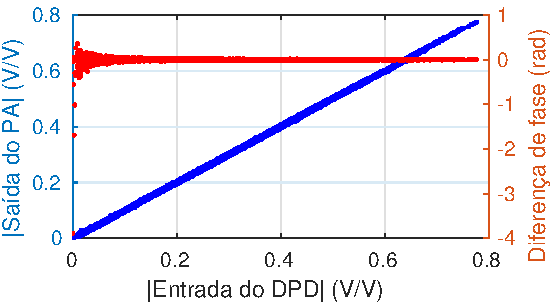
\includegraphics[scale=0.9]{fig2/fig_dpd_ldmos.pdf}
}
\hspace{0.5cm}
\subfloat[GaN{\_}AB{\_}1]{
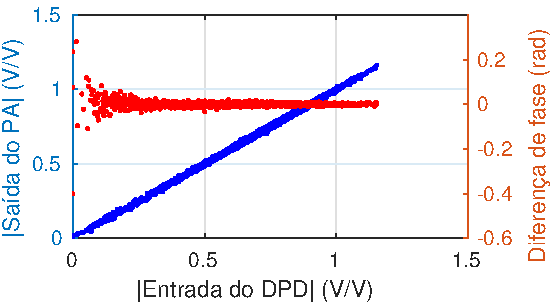
\includegraphics[scale=0.9]{fig2/fig_dpd_sbrt2.pdf}
}
\hspace{0.5cm}
\subfloat[GaN{\_}AB{\_}2]{
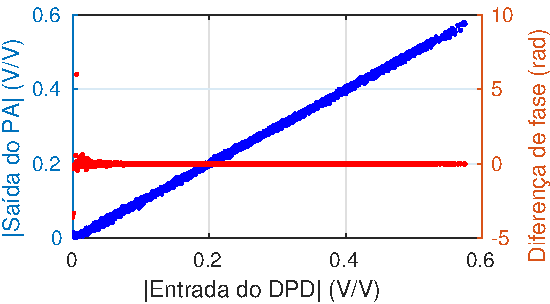
\includegraphics[scale=0.9]{fig2/fig_dpd_tc.pdf}
}
\hspace{0.5cm}
\subfloat[GaN{\_}Doherty]{
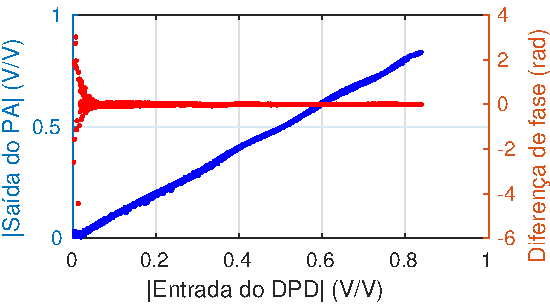
\includegraphics[scale=0.9]{fig2/fig_dpd_doherty.pdf}
}
}{O autor}{fig:bf-dpd}{}{Amplitude de saída do PA e diferença de fase na cascata em função da amplitude de entrada do DPD para os diferentes PAs.}

\imagemHH{Resultados PSD}{
\label{fig:bf-psd}
\subfloat[LDMOS{\_}AB]{
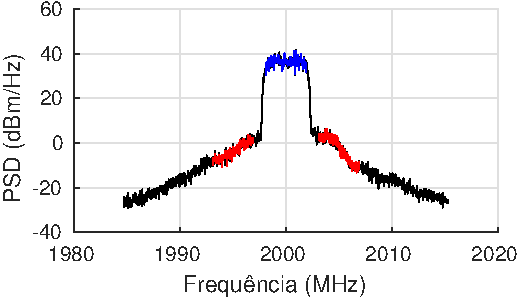
\includegraphics[scale=0.9]{fig2/Frequencia_extraction_ldmos.pdf}
}
\hspace{0.5cm}
\subfloat[GaN{\_}AB{\_}1]{
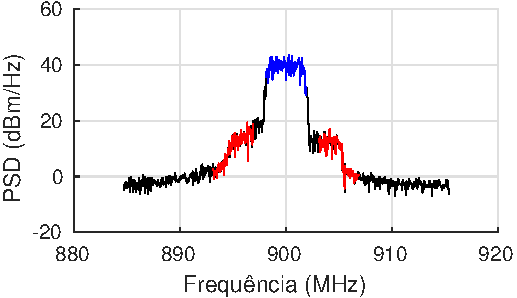
\includegraphics[scale=0.9]{fig2/Frequencia_extraction_sbrt2.pdf}
}
\hspace{0.5cm}
\subfloat[GaN{\_}AB{\_}2]{
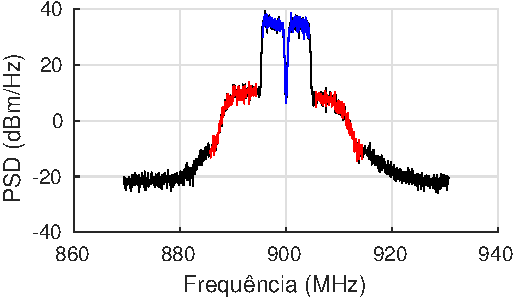
\includegraphics[scale=0.9]{fig2/Frequencia_extraction_tc.pdf}
}
\hspace{0.5cm}
\subfloat[GaN{\_}Doherty]{
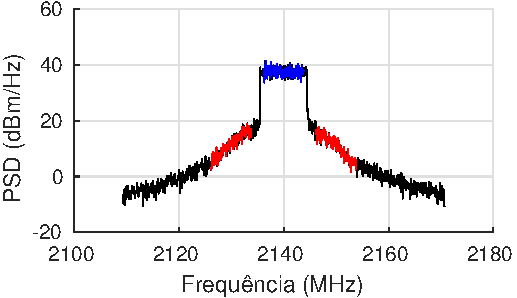
\includegraphics[scale=0.9]{fig2/Frequencia_extraction_doherty.pdf}
}
}{O autor}{fig:bf-psd}{}{PSD para as entradas estimadas dos DPDs e as saídas medidas dos PAs, considerando-se os conjuntos de dados de treinamento.}
